
\begin{figure}[!t!h!b!]
\centering
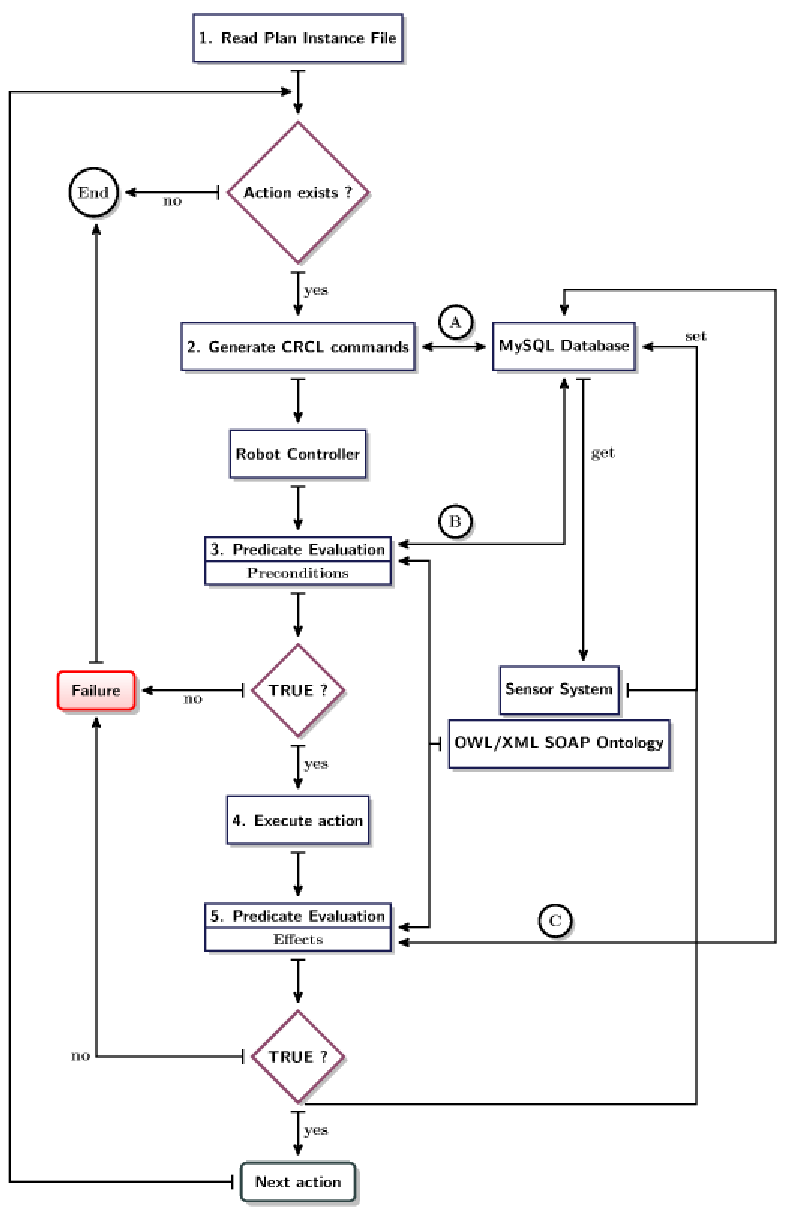
\includegraphics[width=10cm]{images/flowchart.pdf}
\caption{Flowchart diagram for tasking the simulated sensor.}
\label{fig:sensor}
\end{figure}

As seen previously, Section~\ref{subsection:usartruth} describes how a simulated sensor system operates to retrieve 6DOF poses of objects in the kitting workcell. This section describes when the simulated sensor system is used. Figure~\ref{fig:sensor} is a flowchart which represents some of the steps used for kitting, from parsing the \textsf{Plan Instance File} to the execution of each action from this file. Since the focus of this paper is on the sensor system, the authors have limited the representation and description of Figure~\ref{fig:sensor} around the sensor system and did not include the steps prior to the \textsf{Plan Instance File} generation. The reader may find this missing information in the description of Figure~\ref{fig:methodology} in Section~\ref{section:architecture}. The different steps depicted in Figure~\ref{fig:sensor} are categorized into main components that are numbered. A description of each main component is given in the following subsections.

\subsection{Read Plan Instance File}
As described in Section~\ref{section:architecture}, the \textsf{Plan Instance File} is generated by the \textsf{Domain Independant Planning System} from the \textsf{PDDL Domain File} and the \textsf{PDDL Problem File}. An example of a plan is given in Figure~\ref{fig:Solution}. This plan describes the PDDL actions that a robot will need to execute in order to build a kit that consists of one part of type D and one part of type E. At the beginning of the plan (line 1), the end effector that is capable of grasping parts is taken from the end effector changing station and attached to the robot. Lines 2 and 4 display the actions for picking up a part of type E and D, respectively. Lines 3 and 5 display the actions for putting parts E and D in the kit, respectively. Finally, at line 6, the end effector is put back in the end effector changing station.
\begin{figure}[t!h!]
\begin{minipage}{.5\paperwidth}
\begin{list}{}{\setlength{\leftmargin}{0em}}\item\small
\begin{Verbatim}[commandchars=\\\{\},fontsize=\normalsize, numbers=left, numbersep=0pt]
(\opsmall{attach-endeffector} \constsmall{robot_1} \constsmall{part_gripper} \constsmall{part_gripper_holder} \constsmall{changing_station_1})
(\opsmall{take-part} \constsmall{robot_1} \constsmall{part_e1} \constsmall{ptr_e} \constsmall{part_gripper})
(\opsmall{put-part} \constsmall{robot_1} \constsmall{part_e1} \constsmall{kit_a2b3c3d1e1} \constsmall{work_table_1} \constsmall{ptr_e})
(\opsmall{take-part} \constsmall{robot_1} \constsmall{part_d1} \constsmall{ptr_d} \constsmall{part_gripper})
(\opsmall{put-part} \constsmall{robot_1} \constsmall{part_d1} \constsmall{kit_a2b3c3d1e1} \constsmall{work_table_1} \constsmall{ptr_d})
(\opsmall{remove-endeffector} \constsmall{robot_1} \constsmall{part_gripper} \constsmall{part_gripper_holder} \constsmall{changing_station_1})
\end{Verbatim}
\end{list}
\end{minipage}
\caption{Excerpt of the PDDL solution file for kitting.}
\label{fig:Solution}
\end{figure}


\subsection{Generate CRCL Commands}
\label{subsection:CRCL}
Each action of the plan is sequentially interpreted and then directly executed by the robot. The \textsf{Interpreter} takes as input a PDDL action from the \textsf{Plan Instance File} and outputs a set of CRCL commands for this action. To facilitate late binding, the PDDL actions within the plan  do not specify the exact locations of the parts and components that are involved. This kind of knowledge detail is maintained by sensor processing and is stored in the \textsf{MySQL Database}. As described in Section~\ref{section:architecture}, the generation of the tables in the \textsf{MySQL Database} is followed by data insertion in these tables for all the objects in the environment. However, there is no guarantee that the poses of these objects are still accurate as they may have been altered in different ways. At this point, the sensor system is tasked to retrieve information about objects of interest. Objects of interests are the ones for which the poses are needed to execute some CRCL commands. Before tasking the sensor to retrieve the poses of objects of interest via the \textsf{get} message, the external shape of each object of interest must be retrieved from the \textsf{ExternalShape} MySQl table.

An external shape is a shape defined in an external file. An external shape has a model format name, stored in the field \textsf{hasExternalShape\_ModelName}, a model type name, stored in the field \textsf{hasExternalShape\_ModelTypeName}, and a model file name which is the name of the file containing the model, stored in the field \textsf{hasExternalShape\_ModelFileName}. Using the information from retrieved from the aforementioned fields for each object of interest, the system then parses the data coming in from USARTruth and updates the relative pose in the \textsf{MySQL Database} for each object returned. This is a performed via the \textsf{set} message. Since USARTruth returns object locations in global coordinates, the relative pose for each object is updated without changing its transformation tree; that is, the object of reference for its physical location is unchanged. 


The actual updated relative pose is computed according to Equation~\ref{eq:one}.
 \begin{equation}
\label{eq:one}
 L' = LG^{-1}G'
 \end{equation}

where $L'$ is the updated relative transformation, $L$ is the old relative transformation (read from the \textsf{MySQL Database}), $G$ is the old global transformation (computed from the transformation tree in the \textsf{MySQL Database}), and $G'$ is the updated global transformation (retrieved from USARTruth).

Once the above process is performed, the \textsf{Interpreter} uses the new data to generate a set of CRCL commands for the current action, as depicted by \mycirc{A} in Figure~\ref{fig:sensor}. The \op{take-part} action at line 2 in Figure~\ref{fig:Solution} is interpreted as the sequence of CRCL commands displayed in Table~\ref{tab:takepart}, where the numerical data used in the \texttt{MoveTo} commands are computed with the new 6DOF poses. The reader may find more information about the whole set of CRCL commands in~\cite{Balakirsky2012-1}.

\begin{table}[h!]

\caption{A set of CRCL commands for the action \op{take-part}.}
\centering
  \begin{tabular}{l}
    \hline
    \texttt{initCannon()}\\
    \texttt{Message (``take part part\_e1'')}\\
    \texttt{MoveTo(\{\{-0.03, 1.62, -0.25\}, \{0, 0, 1\}, \{1, 0, 0\}\})}\\
    \texttt{Dwell (0.05)}\\
    \texttt{MoveTo(\{\{-0.03, 1.62, 0.1325\}, \{0, 0, 1\}, \{1, 0, 0\}\})} \\
    \texttt{CloseGripper ()} \\
    \texttt{MoveTo(\{\{-0.03, 1.62, -0.25\}, \{0, 0, 1\}, \{1, 0, 0\}\})}\\
    \texttt{Dwell (0.05)}\\
    \texttt{endCannon()}\\
    \hline
  \end{tabular}
  \label{tab:takepart}
\end{table}

Once a set of CRCL commands is generated for a PDDL action, it is sent to the \textsf{Robot Controller} to be executed by the robot. The \textsf{Predicate Evaluation} process is then called before and after each set of CRCL commands is carried out by the robot.

\subsection{Predicate Evaluation (Preconditions)}
As mentioned in Section~\ref{section:architecture}, a PDDL action consists of one precondition section and one effect section that are defined in the \textsf{OWL/XML SOAP Ontology}. Preconditions and effects consist of a set of predicates. For instance, the predicates in the precondition and effect for the action \op{take-part}(\const{robot\_1},\const{part\_e1},\\\const{ptr\_e},\const{part\_gripper}) is defined in Table~\ref{tab:takepartpddl}.


\begin{table}[h!]
\caption{The precondition and the effect for the action \op{take-part}.}
\centering
\begin{tabular}{ l|l }
  \textit{precondition} & \textit{effect} \\
  \hline
  \stvarsmall{part-location-partstray}(\constsmall{part\_e1},\constsmall{ptr\_e})
  &$\neg$\stvarsmall{part-location-partstray}(\constsmall{part\_e1},\constsmall{ptr\_e})\\
  \stvarsmall{robot-empty}(\constsmall{robot\_1})
  & $\neg$\stvarsmall{robot-empty}(\constsmall{robot\_1})\\
  \stvarsmall{endeff-location-robot}(\constsmall{part\_gripper},\constsmall{robot\_1})
  & \stvarsmall{part-location-robot}(\constsmall{part\_e1},\constsmall{robot\_1})\\
  \stvarsmall{robot-with-endeff}(\constsmall{robot\_1},\constsmall{part\_gripper})
  & \stvarsmall{robot-holds-part}(\constsmall{robot\_1},\constsmall{part\_e1})\\
  \stvarsmall{endeff-type-part}(\constsmall{part\_gripper},\const{part\_e1})
  &  \\
  \stvarsmall{partstray-not-empty}(\constsmall{ptr\_e})
  &
\end{tabular}
  \label{tab:takepartpddl}
\end{table}

\subsubsection{Spatial Relations -- }
 The evaluation of the predicates in the precondition section assures that all the requirements are met in the environment before the robot carries out the action. As such, the output of the \textsf{Predicate Evaluation} process is a Boolean value. The kitting system relies on the representation of spatial relations that are stored in the \textsf{OWL/XML SOAP Ontology} to compute the truth-value of each predicate. A brief description of each spatial relation is given below. A thorough analyze of spatial relations used for kitting is well documented in~\cite{SCHLENOFF.RAS.2013}. 
\begin{itemize}
 \item Predicates: These are domain-specific states that are of interest to the current domain. The truth-value of predicates can be determined through the logical combination of intermediate state relations.
\item Intermediate state relations: These are intermediate level state relations that can be inferred from the combination of RCC8 and cardinal direction relations.
\item RCC8 relations: Region Connected Calculus (RCC8)~\cite{Wolter2000} is a well-known and cited approach for representing the relationship between two regions in Euclidean space or in a topological space. RCC8 was initially developed for a two-dimensional space but has been extended for the purpose of the kitting effort to a three-dimensions space by applying it along all three planes (x-y, x-z, y-z). Each of the intermediate state relations consists of a set of logical rules that associate these RCC8 relations to them. There are 24 RCC8 relations and 6 cardinality direction operators.
\end{itemize}

\subsubsection{Sensor System -- }
To evaluate the truth-value of any given predicate, the sensor system is tasked to retrieve the 6DOF of the predicate's parameters. This is performed the same way it is described in Section~\ref{subsection:CRCL} and is represented by \mycirc{B} in Figure~\ref{fig:sensor}. The \textsf{Predicate Evaluation} process then proceeds as follows:

%The predicates developed for the kitting effort have at least one parameter and at most two parameters. In the case the predicate has two parameters, the external shape of each parameter is fetched from the \textsf{MySQL Database} and is passed to USARTruth to get the pose information of each object. The \textsf{Predicate Evaluation} process then proceeds as follows:
\begin{itemize}
\item[] In the \textsf{OWL/XML SOAP Ontology}:
\begin{enumerate}
 \item Identify the predicate.
 \item Identify the intermediate state relation for the predicate from step 1.
 \item Identify the set of logical rules that associate RCC8 relations to the intermediate state relation from step 2.
\end{enumerate}
\end{itemize}

\subsubsection{RCC8 Evaluation -- }
Next, the poses of the predicate's parameters are used to compute the truth-value of the identified set of logical rules of RCC8 relations for this predicate. The predicates developed for the kitting effort have at least one parameter and at most two parameters. To evaluate the set of RCC8 relations, two methods are used. 


\begin{enumerate}
\item In the case the predicate has two parameters, the poses of these two parameters are used to compute the truth-value of the set of RCC8 relations. For instance, the predicate \stvar{part-location-partstray}(\const{part\_e1},\const{ptr\_e}) from Table~\ref{tab:takepartpddl} is true iff the part \const{part\_e1} is partially in the parts tray \const{ptr\_e}. The two objects involved for this predicate are the parameters of the predicate. The intermediate state relation associated to this predicate is defined in formula~\ref{formula:partiallyin1}.


\begin{gather}
\label{formula:partiallyin1}
\textbf{Partially-In}(\textit{part\_e1}, \textit{ptr\_e}) \rightarrow   \\
(\texttt{Z-Plus}(\textit{part\_e1}, \textit{ptr\_e}) \wedge (\texttt{Z-NTPP}(\textit{part\_e1}, \textit{ptr\_e}) \vee \texttt{Z-NTPPi}(\textit{part\_e1}, \textit{ptr\_e}) \vee  \notag\\\texttt{Z-PO}(\textit{part\_e1}, \textit{ptr\_e}) \vee \texttt{Z-TPP}(\textit{part\_e1}, \textit{ptr\_e}) \vee \texttt{Z-TPPi}(\textit{part\_e1}, \textit{ptr\_e}))) \wedge \notag\\
(\texttt{X-NTPP}(\textit{part\_e1}, \textit{ptr\_e}) \vee \texttt{X-NTPPi}(\textit{part\_e1}, \textit{ptr\_e}) \vee \texttt{X-TPP}(\textit{part\_e1}, \textit{ptr\_e}) \vee  \notag\\ \texttt{X-TPPi}(\textit{part\_e1}, \textit{ptr\_e}))\wedge
(\texttt{Y-NTPP}(\textit{part\_e1}, \textit{ptr\_e}) \vee \texttt{Y-NTPPi}(\textit{part\_e1}, \textit{ptr\_e}) \vee  \notag\\ \texttt{Y-TPP}(\textit{part\_e1}, \textit{ptr\_e}) \vee \texttt{Y-TPPi}(\textit{part\_e1}, \textit{ptr\_e})) \notag
\end{gather}

\item In the case the predicate has only one parameter, a second object is needed to compute the truth-value of the predicate between the parameter and the other object. The authors remind the reader that RCC8 relations necessarily require two objects. In this case, the sensor system is tasked to retrieve the pose for each other object in the workcell to be used as the second object. Depending on the predicate, the search space for the other object can be narrowed down. For instance, the predicate \stvar{partstray-not-empty}(\const{ptr\_e}) (Table~\ref{tab:takepartpddl}) is true iff at least one part of type E is in the parts tray \const{ptr\_e}. It is not necessary to extend the search for the second object among the other types of object present in the workcell. It is not relevant for instance to check if the parts tray contains an end effector. On the other hand, to check the truth value of the predicate \stvar{robot-empty}(\const{robot\_1}) (Table~\ref{tab:takepartpddl}), which is true iff the robot \const{robot\_1} is not holding anything in the end effector attached to the robot, the predicate evaluation needs to scan a wider search space than the one described for the predicate \stvar{partstray-not-empty}(\const{ptr\_e}), i.e., the search space includes all parts of each type, all types of kit trays, etc. 

Once the search space has been defined, the external shape for each object in the search space is retrieved from the appropriate table from the \textsf{MySQL Database}. As described previously, the external shape is used by the sensor system to retrieve the 6DOF pose for the corresponding object. The truth-value of the set of logical rules that associate RCC8 relations to the intermediate state relation for the predicate is then computed for these two objects, that is the predicate parameter and the searched object. 
%To illustrate the case where predicates have only one parameter, formula~\ref{formula:partiallyin2} is used as an example.
%
%The intermediate state relation associated to this predicate is is defined in formula~\ref{formula:partiallyin2}.

%\begin{gather}
%\label{formula:partiallyin2}
%\textbf{Partially-In}(\textit{ptr\_e}, \textit{$obj_2$}) \rightarrow   \\
%(\texttt{Z-Plus}(\textit{ptr\_e}, \textit{$obj_2$}) \wedge (\texttt{Z-NTPP}(\textit{ptr\_e}, \textit{$obj_2$}) \vee \texttt{Z-NTPPi}(\textit{ptr\_e}, \textit{$obj_2$}) \vee  \notag\\\texttt{Z-PO}(\textit{ptr\_e}, %\textit{$obj_2$}) \vee \texttt{Z-TPP}(\textit{ptr\_e}, \textit{$obj_2$}) \vee \texttt{Z-TPPi}(\textit{ptr\_e},\textit{$obj_2$}))) \wedge \notag\\
%(\texttt{X-NTPP}(\textit{ptr\_e},\textit{$obj_2$}) \vee \texttt{X-NTPPi}(\textit{ptr\_e},\textit{$obj_2$}) \vee \texttt{X-TPP}(\textit{ptr\_e},\textit{$obj_2$}) \vee  \notag\\ \texttt{X-TPPi}(\textit{ptr\_e},%\textit{$obj_2$}))\wedge
%(\texttt{Y-NTPP}(\textit{ptr\_e},\textit{$obj_2$}) \vee \texttt{Y-NTPPi}(\textit{ptr\_e},\textit{$obj_2$}) \vee  \notag\\ \texttt{Y-TPP}(\textit{ptr\_e},\textit{$obj_2$}) \vee \texttt{Y-TPPi}(\textit{ptr\_e},%\textit{$obj_2$})) \notag
%\end{gather}
\end{enumerate}
%
%For instance, to evaluate the predicate \stvar{part-location-partstray}(\const{part},\const{partstray}), the external shapes for \const{part} and \const{partstray} are retrieved from the \textsf{MySQL Database} and their %poses are retrieved by USARTruth. Those poses are then used by a combination of spatial relations to compute the truth-value of this predicate.

%In the case the predicate has only one parameter, \stvar{robot-empty}(\const{robot}) for instance, the external shape of this parameter is used by USARTruth to retrieve this parameter's pose from USARSim (pose of %\const{robot} in this example). Since the computation of spatial relations always requires two objects, the external shape, thus the pose of each single other object in the environment is retrieved and used as the second %object.

If all the predicates within the precondition section are true, the \textsf{MySQL Database} is updated with the current poses of these predicates' parameters. It is important that all the predicates are true in order to update the \textsf{MySQL Database}. This ensures that a complete (stable) state of the environment is stored in the \textsf{MySQL Database}. If at least one predicate is evaluated to false, it is considered a failure and the kitting process is terminated.

\subsection{Execute Action}
When all the predicates within the precondition of an action have been evaluated to true, this action is executed by the robot. To confirm that the action was successfully accomplished, the \textsf{Predicate Evaluation} process evaluates the predicates within the effect section for this action. The effect section consists of predicates that are expected to be true after performing a PDDL action. The evaluation of the predicates within the effect section is performed to confirm that these expectations are attained.

\subsection{Predicate Evaluation (Effects)}
The methodology previously described to evaluate the predicates within the precondition section of an action is also used to evaluate the predicates within the effect section of this action. This is depicted by \mycirc{C} in Figure~\ref{fig:sensor}. As mentioned earlier, all the predicates within the effect section must be evaluated to true to define the action as successful. In the case of a successful action, the next action within the \textsf{Plan Instance File} is processed. Once all the actions within the \textsf{Plan Instance File} have been executed by the robot, the kitting process is complete.
% <<<<<<< HEAD
% \section{The Virtual Sensor System}
% \label{sec:sensor}
% This section is an extension of Section~\ref{sect:architecture}. The focus of this section is on the methodology that is used to task the virtual sensor system to retrieve 6DOF pose estimation of objects of interest in the kitting work cell. Figure~\ref{fig:methodology} is often mentioned. To facilitate the understanding of the description given in this section, we refer to components in Figure~\ref{fig:methodology} by the term \texttt{design(x,y)} where \texttt{x} represents one of the x axis level (i.e., Sense, Model, and Act) and \texttt{y} represents one of the y axis level (i.e., Domain Specific Information, Ontology, Planning Language, and Robot Language).
% 
% 
% \subsection{Methodology for Tasking the Virtual Sensor System}
% \label{sec:sensor-1}
% As depicted in Figure~\ref{fig:methodology} (\texttt{design(Sense, Domain Specific Information)}), the Sensor Processing is called during the Predicate Evaluation process. As described in Section~\ref{sect:architecture}, a PDDL action consists of preconditions and effects. Preconditions and effects consist of a set of predicates and each predicate consists of variables (objects of interest). 
% 
% %As seen at the Robot Language level, the interpreter takes a PDDL plan as input and generates a CRCL plan which consists of low level robot commands. These robot commands are then read by the Robot Controller to be executed (\texttt{design(Act, Robot Language)}). 
% 
% 
% As seen at the Robot Language level, the interpreter takes the plan file as input and builds the corresponding CRCL file. Real time information on the environment is required in order to fill in information required by the CRCL on
% object locations. Since both the OWL and XML implementations of the knowledge representation are file based, real time information proved to be problematic. In order to solve this problem,
% an automatically generated MySQL database \cite{MySQL} has been introduced as part of the knowledge representation.
% Table~\ref{tab:takepart} shows an example of CRCL commands generated for the PDDL action \stvar{take-part(part\_b\_1)}. Please note that the PDDL action \stvar{take-part} developed for the current kitting domain has more than one parameter. Not all the parameters are relevant for the example depicted in Table~\ref{tab:takepart} and the number of parameters has been  reduced for simplicity. In this example,
% the locations of the \lq\lq{}MoveTo\rq\rq{} commands would come from the MySQL database.
% 
% \begin{table}[h!]
% \centering
% 
%     \begin{tabular}{l}
%     \stvar{take-part(part\_b\_1)}\\
%     \hline
%     \hline
%   \texttt{\scriptsize{Message (``take part part\_b\_1")}}\\
%   \texttt{\scriptsize{MoveTo(\{\{-0.03, 1.62, -0.25\}, \{0, 0, 1\}, \{1, 0, 0\}\})}}\\
%   \texttt{\scriptsize{Dwell (0.05)}}\\
%   \texttt{\scriptsize{MoveTo(\{\{-0.03, 1.62, 0.1325\}, \{0, 0, 1\}, \{1, 0, 0\}\})}} \\
%   \texttt{\scriptsize{CloseGripper ()}} \\
%   \texttt{\scriptsize{MoveTo(\{\{-0.03, 1.62, -0.25\}, \{0, 0, 1\}, \{1, 0, 0\}\})}}\\
%   \texttt{\scriptsize{Dwell (0.05)}}\\
%   \hline
%   \end{tabular}
% \caption{An example of CRCL commands for a PDDL action}
%   \label{tab:takepart}
% \end{table}
% 
% After the execution of a set of robot commands corresponding to a single PDDL action, the System Monitor triggers the Predicate Evaluation process (\texttt{design(Sense, Domain Specific Information)}). The Predicate Evaluation process examines the predicates that consist the effects for the executed PDDL action. Note that we don't describe how the system traces back from the CRCL plan to the PDDL plan in order to identify the PDDL action that has just been carried. This process is described in another paper~\cite{Balakirsky.RITA.2013} that was submitted in the same special session. In order to validate the predicate for the action's effects, the virtual sensor system is tasked to retrieve the ground truth for the variables of each predicate in the effects section. A detailed description of how predicates are evaluated can be found in~\cite{Balakirsky2013}. 
% 
% Once the Predicate Evaluation process is performed, a new process calls the MYSQL Interface Library (\texttt{design(Model, Planning Language)}) to update the MySQL database with the 6DOF pose estimation for the objects of interest. Please note that the poses coming from the virtual sensor system are in global coordinates while the poses of objects in the MySQL database are in local coordinates. The transformation from one reference frame to the other is described in the next section.
% 
% 
% \subsection{The Virtual Sensor Tool}
% While the previous section described the methodology used to task the virtual sensor during kitting, this section presents a technical description of the tool used to simulate the sensor system.
% 
% USARSim can be directly queried to return the 6DOF pose of a specific object, or of every object of a certain type. The simulator USARTruthConnection object listens for incoming connections on port 3989, and receives queries over a socket in the form of strings formatted into key-value pairs. The USARTruth connection accepts two different keys, ``class'' and ``name,'' which are both optional. When USARSim receives a new string over the connection, it sends a sequence of key-value formatted strings back over the socket, one for each Unreal Engine Actor object that matches the requested class and object names. The return strings include the following keys:
% 
% \begin{itemize}
% \item Name: The internal name of the object in USARSim.
% \item Class: The name of the most specific Unreal Engine class the object belongs to.
% \item Time: The number of seconds that have elapsed since the simulator start, as a floating-point value.
% \item Location: The comma-separated position of the object in global coordinates.
% \item Rotation: The comma-separated orientation of the object in global coordinates, in roll, pitch, yaw form.
% \end{itemize}
% 
% The virtual sensor system uses USARTruth to simulate real-world sensors by opening a new USARTruth connection and sending one request for each different Unreal Engine class name found in the MySQL database. For simulation purposes, the Unreal Engine class name is stored as an object's ``external shape''. It is important to note that the Location and Rotation values coming out of USARTruth do not include noises and assume perfect sensor data.
% 
% The system then parses the data coming in from USARTruth and updates the relative pose in the MySQL database for each object returned. Since USARTruth returns object locations in global coordinates, the relative pose for each object is updated without changing its transformation tree; that is, the RefObject for its PhysicalLocation is unchanged. The actual updated relative pose is computed according to
% \begin{equation}
% L' = LG^{-1}G'
% \end{equation}
% where $L'$ is the updated relative transformation, $L$ is the old relative transformation (read from the MySQL database), $G$ is the old global transformation (computed from the transformation tree in the database), and $G'$ is the updated global transformation (retrieved from USARTruth).
% =======
% \section{Failure Analysis}
% As seen in Figure~\ref{fig:predicateEval}, failures are identified during the evaluation of preconditions and effects. 
% In addition to recognizing failures, it is desired to be able to respond to them.
% In order to properly model this response, additional information must be modeled
% in the ontology. As shown in Figure \ref{fig:failure}, the class {\it ActionFailureType} has been added to the ontology. This class is composed of a {\it PredicateType} class and a {\it FailureModeType} class. It contains all of the information required to be able to diagnose and remediate any failures that are detected by the system.
% 
% The {\it PredicateType} class contains a list of predicates whose truth values caused the detection of the current failure condition. Examination of the instances pointed to by the {\it ReferenceParameter} and the {\it TargetParameter} allow the system to understand exactly which components were involved in the failure.
% 
% The {\it FailureModeType} class provides various known failure modes that could exist for the combination of {\it PredicateType}s that were found deficient. It provides the consequences of such a failure occurring, information on how to remediate such a failure, and the chance that this kind of failure could occur. Understanding the consequences of the failure mode is important if one would like to be able to
% pinpoint the correct cause of the failure. For example, assume that the action {\sc take-part} failed, and the predicate that indicated the failure was {\it part-in-gripper}. Understanding where the part is actually located is critical to understanding the root cause of the failure. If the part is still in the parts tray, it would indicate a grasp related failure. If the part is on the floor of the cell, it would indicate a part handling error. This kind of information is represented in the {\it Effect} class of the consequences. Being able to pinpoint the effects of the failure also allows for judgment on the failure severity. A missed grasp will likely lead to a new grasp attempt and will have little impact on operation. A dropped part may cause damage to the part and have a higher severity level.
% 
% Failure remediation is described by the {\it FailureRemediation} class. This class contains information on what notifications need to be sent as a result of the failure as well as what actions should be taken. Continuing our example from above, the grasp failure may cause grasping information to be sent to the enginering department for algorithm development while the dropped part may notify logistics that an additional component will be required. Recovery from the failure is possible by executing the {\it Plan} that accompanies the detected failure.
% >>>>>>> 30bc69f3bb5ccebcc52647c51ed3b2fe4e707ac9
